%!TEX program = lualatex

%\documentclass[OA,linenum,doublespace]{InterPore}
%\documentclass[OA,linenum,suppleart]{InterPore}
%\documentclass[OA,linenum,suppleart,CCBY]{InterPore}
%\documentclass[OA,linenum,CCBY]{InterPore}
%\documentclass[OA,linenum]{nbr_article}
\documentclass[OA]{nbr_article}

\artcategory{Original Research}

%%%%%%%%%%%%%%%%%%%%%%%%%%%%%%%%%%%%%%%%%%%%%%%%%%%%%%%%%%%%%%%%%%%%%%%%%
%%% The following information will be updated by the Editorial Office %%%
%%%%%%%%%%%%%%%%%%%%%%%%%%%%%%%%%%%%%%%%%%%%%%%%%%%%%%%%%%%%%%%%%%%%%%%%%
\vol{0}
\iss{0}
\cpyear{2026 Under Review} 
\doi{00.0000/000000000}
\recdate{00 Month 0000}
\accdate{01 Month 0000}
\pubdate{02 Month 0000}
\rhauthor{Last Name First Author, et al.}
\citethisarticle{This information will be updated by the Editorial Office once the article is ready to be published. \url{https://doi.org/10.69631/xxxxxxx}}

% Optional:
% \CCbystatement{Creative Commons Attribution 4.0 International license (CC BY 4.0 Deed) \url{https://creativecommons.org/licenses/by/4.0/}}
% \CPstatement{© \the\year\ Customized\newline CP statement}

%%%%%%%%%%%%%%%%%%%%%%%%%%%%%%%%%%%%%%%%%%%%%%%%%%%%%%%%%%%%%%%%%%%%%%%%%
%%%                     End Editorial Office                          %%%
%%%%%%%%%%%%%%%%%%%%%%%%%%%%%%%%%%%%%%%%%%%%%%%%%%%%%%%%%%%%%%%%%%%%%%%%%

\graphicspath{
	{./Figures/}
	{./logo/}
}

\begin{document}
	
	
	%%%%%%%%%%%%%%%%%%%%%%%%%%%%%%%%%%%%%%%%%%%%%%%%%%%%%%%%%%%%%%%%%%%%%%%%%
	%%%                     Begin author content                          %%%
	%%%%%%%%%%%%%%%%%%%%%%%%%%%%%%%%%%%%%%%%%%%%%%%%%%%%%%%%%%%%%%%%%%%%%%%%%
	\title{A Descriptive Title Goes Here and Can Span Multiple Lines if Needed}
	
	\author[1\orc{0000-0000-0000-0001}]{First Author}
	\author[1\orc{0000-0000-0000-0002}]{Second Author}
	\author[2\orc{0000-0000-0000-0003}]{Third Author}
	\author[4\orc{0000-0000-0000-0004}]{Fourth Author}
	\author[1\orc{0000-0000-0000-0005}]{Fifth Author}
	\author[2\orc{0000-0000-0000-0006}]{Sixth Author}
	\author[3\orc{0000-0000-0000-0007}]{Seventh Author}
	\author[4\orc{0000-0000-0000-0008}]{Eighth Author}
	
	\affil[1]{First Affiliation} %
	\affil[2]{Second Affiliation} %
	\affil[3]{Third Affiliation} 
	\affil[4]{Fourth Affiliation\vspace*{-4pt}} 
	
	\corau{Correspondence Author Name, \email{Correspondence Author Email} Optional Affiliation}
	
	\abstract{The abstract should provide a concise and informative summary of the manuscript. It should include the following key components: a clear statement of the study’s purpose or research question; a brief description of the methods used, including experimental, theoretical, or analytical approaches; a summary of the main results and how they address the research question; conclusions outlining the implications of the findings and their relevance to porous media research; and a statement of the study’s significance, highlighting its contribution to the existing body of knowledge and its broader impact or applications. This paragraph serves as placeholder text to illustrate the expected structure, length, and content of an abstract within the manuscript template. 
		%%%NOTE%%%
		% must add skip or space or enough text 
		% otherwise copyright overlaps text
		\vskip 1cm
	}
	
	\keyword{Provide up to 6 or 7 keywords or phrases}
	
	\maketitle
	
	\section{First Level Head}
	
	\lipsum[1-2]
	\begin{wrapfigure}{r}{200pt}
		\centering
		\fbox{%
			\begin{minipage}{172pt} % box width
				\centering
				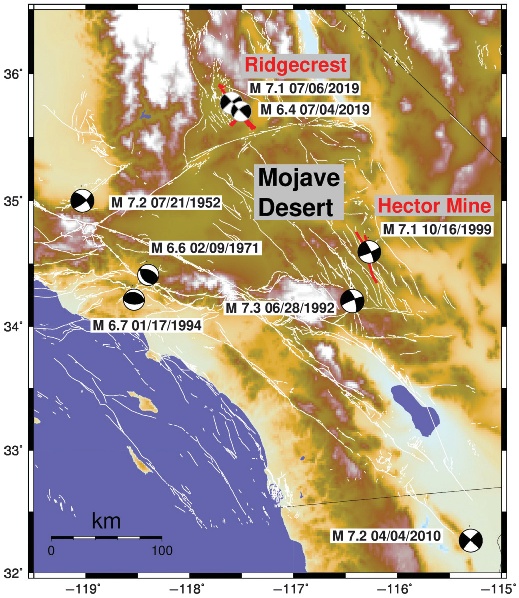
\includegraphics[width=172pt]{Figures/Sample}
				\captionof{figure}{Figure caption goes here. a) Figure caption goes here and provides a brief description of the illustration. Figure caption goes here and explains the main elements shown in the figure. b) Figure caption goes here to indicate how different cases or panels may be interpreted. Figure caption goes here to describe relationships, trends, or schematic features presented. d) Figure caption goes here.}
				\label{fig01}
			\end{minipage}%
		}
	\end{wrapfigure}
	%
	\lipsum[8-9]
	%
	\subsection{Second Level Head}
	%
	\lipsum[10-12]
	%
	\begin{wrapfigure}{l}{215pt}
		\centering
		\fbox{%
			\begin{minipage}{190pt} % box width
				\centering
				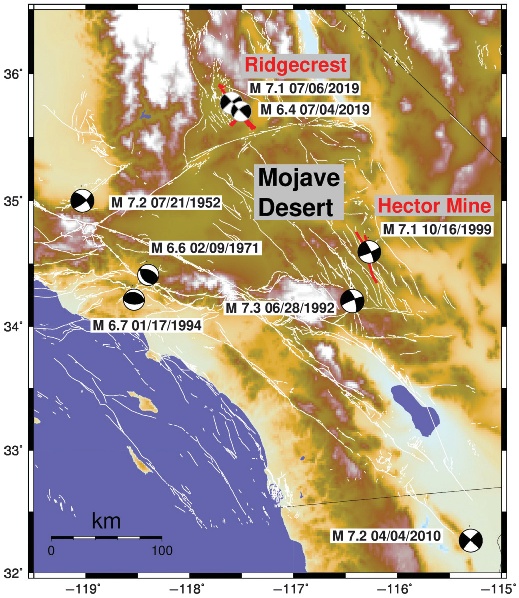
\includegraphics[width=190pt]{Figures/Sample}
				\captionof{figure}{Figure caption goes here. a) Figure caption goes here and provides a brief description of the illustration. Figure caption goes here and explains the main elements shown in the figure.}
				\label{fig02}
			\end{minipage}%
		}
	\end{wrapfigure}
	%
	\lipsum[13-15]
	%
	
	\begin{figure}
		\centering
		\fbox{%
			\begin{minipage}{307pt} % box width
				\centering
				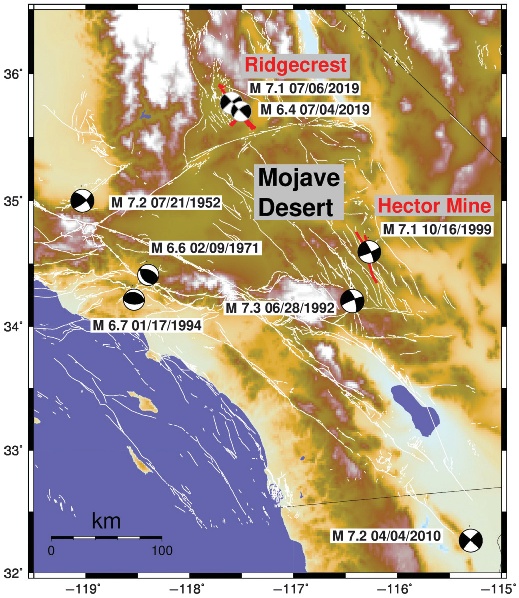
\includegraphics[width=307pt]{Figures/Sample}
				\captionof{figure}{Figure caption goes here. a) Figure caption goes here and provides a brief description of the illustration. Figure caption goes here and explains the main elements shown in the figure. b) Figure caption goes here to indicate how different cases or panels may be interpreted. Figure caption goes here to describe relationships, trends, or schematic features presented. d)  Figure caption goes here.}
				\label{fig03}
			\end{minipage}%
		}
	\end{figure}
	
	
	\begin{table}
		\tbl{Table Caption Goes Here. Table Caption Goes Here. Table Caption Goes Here.\label{tab01}}
		{\begin{tabular}{R l R d{4,0} R l R l R l R} % {\textwidth}\extracolsep{\fill}
				\rowrule
				\TCH\textbf{Complete Dataset} & \multicolumn{1}{c|}{\textbf{N}} &
				\multicolumn{3}{c|}{\textbf{${\sigma}$}}\\ %
				%\cline{3-5}
				\cmidrule(lr){3-5}
				\TCH&& \multicolumn{1}{c|}{\textbf{a}} & \multicolumn{1}{c|}{\textbf{b}} & \multicolumn{1}{c|}{\textbf{c}}\\ %
				\rowrule%
				\multicolumn{5}{|l|}{{a. Faulting Type}} \\ \rowrule%
				{Thrust} & 3801 & 18.1 \% & 0.3 \% & 15.6 \%\\ \rowrule%
				{Strike-Slip} & 3829 & 25.2 \% & 0.3 \% & 18.5 \% \\ \rowrule%
				{Normal} & 3180 & 25.5 \% & 0.4 \% & 19.8 \%\\ \rowrule%
				{Oblique} & 2046 & 25.5 \% & 0.5 \% & 21.0 \%\\ \rowrule%
				\multicolumn{5}{|l|}{{b. Geologic Environment}}\\ \rowrule%
				{Subduction Zone} & 8691 & 21.6 \% & 0.2 \% & 19.7 \% \\ \rowrule%
				{Spreading Center} & 2785 & 28.0 \% & 0.4 \% & 18.2 \% \\ \rowrule%
				{Volcanoes} & 163 & 26.0 \% & 1.6 \% & 20.0 \% \\
				\rowrule
		\end{tabular}}
		{}
	\end{table}
	
	%
	\begin{table}
		\tbl{This is a Sample Table Caption. This is a Sample Table Caption. This is a Sample Table Caption. This is a Sample Table Caption. This is a Sample Table Caption.\label{tab02}}
		{\begin{tabular}{@{}R l R l R l R l R l R l R l R l R l R@{}} %
				\rowrule
				\TCH\textbf{Complete Dataset} & \multicolumn{1}{c|}{\textbf{N}} & \multicolumn{1}{c|}{\textbf{${\mu}$}} & \multicolumn{1}{c|}{\textbf{${\sigma}_{{\mu}}$}} & \multicolumn{1}{c|}{\textbf{${\sigma}$}} & \multicolumn{1}{c|}{\textbf{N}} & \multicolumn{1}{c|}{\textbf{${\mu}$}} & \multicolumn{1}{c|}{\textbf{${\sigma}_{{\mu}}$}} & \multicolumn{1}{c|}{\textbf{${\sigma}$}}\\ %\rowrule%
				% \multicolumn{1}{l}{} & \textbf{12856} & \textbf{23.2 \%} & \textbf{0.2 \%} & \textbf{18.8 \%} \\ %
				\rowrule
				\multicolumn{9}{|l|}{{a. Faulting Type}} \\ \rowrule%
				{Thrust} & 3801 & 18.1 \% & 0.3 \% & 15.6 \% & 3801 & 18.1 \% & 0.3 \% & 15.6 \%\\ \rowrule%
				{Strike-Slip} & 3829 & 25.2 \% & 0.3 \% & 18.5 \% & 3801 & 18.1 \% & 0.3 \% & 15.6 \%\\ \rowrule%
				{Normal} & 3180 & 25.5 \% & 0.4 \% & 19.8 \% & 3801 & 18.1 \% & 0.3 \% & 15.6 \%\\ \rowrule%
				{Oblique} & 2046 & 25.5 \% & 0.5 \% & 21.0 \% & 3801 & 18.1 \% & 0.3 \% & 15.6 \%\\ \rowrule%
				\multicolumn{9}{|l|}{{b. Geologic Environment}}\\ \rowrule%
				{Subduction Zone} & 8691 & 21.6 \% & 0.2 \% & 19.7 \% & 3801 & 18.1 \% & 0.3 \% & 15.6 \%\\ \rowrule%
				{Spreading Center} & 2785 & 28.0 \% & 0.4 \% & 18.2 \% & 3801 & 18.1 \% & 0.3 \% & 15.6 \%\\ \rowrule%
				{Volcanoes} & 163 & 26.0 \% & 1.6 \% & 20.0 \% & 3801 & 18.1 \% & 0.3 \% & 15.6 \%\\ \rowrule%
				\multicolumn{9}{|l|}{{a. Faulting Type}} \\ \rowrule%
				{Thrust} & 3801 & 18.1 \% & 0.3 \% & 15.6 \% & 3801 & 18.1 \% & 0.3 \% & 15.6 \%\\ \rowrule%
				{Strike-Slip} & 3829 & 25.2 \% & 0.3 \% & 18.5 \% & 3801 & 18.1 \% & 0.3 \% & 15.6 \%\\ \rowrule%
				{Normal} & 3180 & 25.5 \% & 0.4 \% & 19.8 \% & 3801 & 18.1 \% & 0.3 \% & 15.6 \%\\ \rowrule%
				{Oblique} & 2046 & 25.5 \% & 0.5 \% & 21.0 \% & 3801 & 18.1 \% & 0.3 \% & 15.6 \%\\ \rowrule%
				\multicolumn{9}{|l|}{{b. Geologic Environment}}\\ \rowrule%
				{Subduction Zone} & 8691 & 21.6 \% & 0.2 \% & 19.7 \% & 3801 & 18.1 \% & 0.3 \% & 15.6 \%\\ \rowrule%
				{Spreading Center} & 2785 & 28.0 \% & 0.4 \% & 18.2 \% & 3801 & 18.1 \% & 0.3 \% & 15.6 \%\\ \rowrule%
				{Volcanoes} & 163 & 26.0 \% & 1.6 \% & 20.0 \% & 3801 & 18.1 \% & 0.3 \% & 15.6 \%\\ \rowrule%
				\multicolumn{9}{|l|}{{a. Faulting Type}}\\ \rowrule%
				{Thrust} & 3801 & 18.1 \% & 0.3 \% & 15.6 \% & 3801 & 18.1 \% & 0.3 \% & 15.6 \%\\ \rowrule%
				{Strike-Slip} & 3829 & 25.2 \% & 0.3 \% & 18.5 \% & 3801 & 18.1 \% & 0.3 \% & 15.6 \%\\ \rowrule%
				{Normal} & 3180 & 25.5 \% & 0.4 \% & 19.8 \% & 3801 & 18.1 \% & 0.3 \% & 15.6 \%\\ \rowrule%
				{Oblique} & 2046 & 25.5 \% & 0.5 \% & 21.0 \% & 3801 & 18.1 \% & 0.3 \% & 15.6 \%\\ \rowrule%
				{Volcanoes} & 163 & 26.0 \% & 1.6 \% & 20.0 \% & 3801 & 18.1 \% & 0.3 \% & 15.6 \%\\
				\rowrule
		\end{tabular}}
		{}
	\end{table}
	
	\lipsum[13-20]
	%
	\begin{figure}
		\centering
		\fbox{%
			\begin{minipage}{\textwidth} % box width
				\centering
				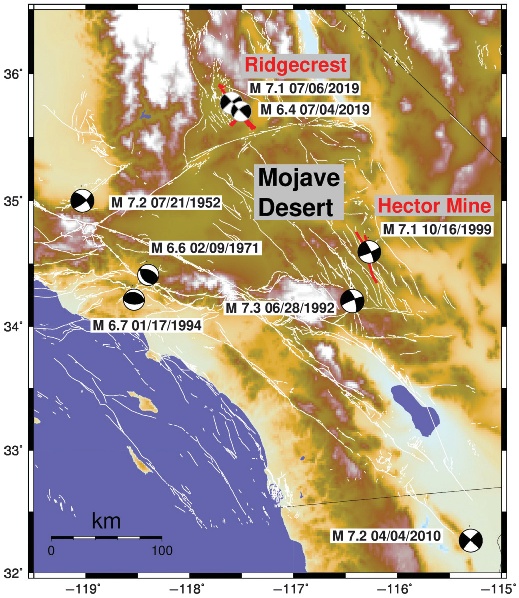
\includegraphics[width=439pt,height=168pt]{Figures/Sample}
				\captionof{figure}{Figure caption goes here. a) Figure caption goes here and provides a brief description of the illustration. Figure caption goes here and explains the main elements shown in the figure. Figure caption goes here to describe relationships, trends, or schematic features presented. d)  Figure caption goes here.}
				\label{fig04}
			\end{minipage}%
		}
	\end{figure}
	
	
	\lipsum[21]
	
	%
	\section{Sample First Level Section Stacked with Second Level}
	\subsection{Second Level Head}
	\subsubsection{Third Level Head}
	
	\lipsum[22]
	\begin{eqnarray}
		u_{\rm mod} ( t ) &=&   a_1^{\rm foreshock} H ( t - t_{\rm foreshock} )  + a_1^{\rm mainshock} H ( t - t_0 )\nonumber\\
		&&{} + a_2 + a_3 ( t - t_0 ) + a_4 \cos ( 2 \pi t ) + a_5 \sin ( 2 \pi t )\nonumber \\
		&&{} + a_6 \cos ( 4 \pi t ) + a_7 \sin ( 4 \pi t ) + u_{\rm post} ( t )
		\label{eqn01}
	\end{eqnarray}
	%
	\lipsum[23-26]
	
	%
	\begin{figure}[!b]
		\centering
		\fbox{%
			\begin{minipage}{\textwidth} % box width
				\centering
				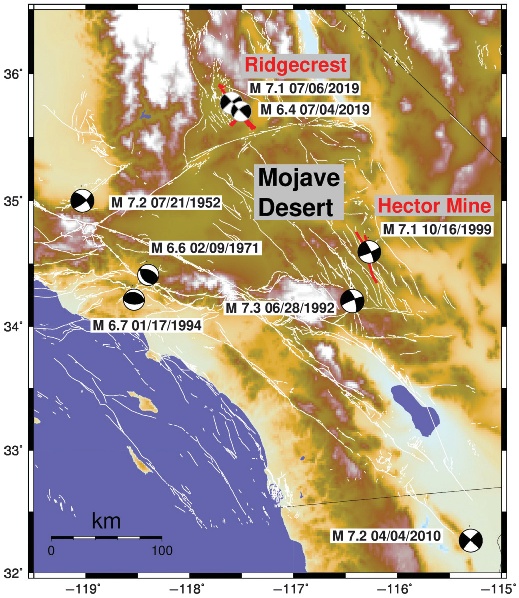
\includegraphics[width=439pt,height=168pt]{Figures/Sample}
				\captionof{figure}{Figure caption goes here. a) Figure caption goes here and provides a brief description of the illustration. Figure caption goes here and explains the main elements shown in the figure. b) Figure caption goes here to indicate how different cases or panels may be interpreted. Figure caption goes here to describe relationships, trends, or schematic features presented. d)  Figure caption goes here.}%
				\label{fig05}%
				%\end{minipage}%
				\bigskip
				\par%
				%\begin{minipage}{\textwidth} % box width
				%\centering
				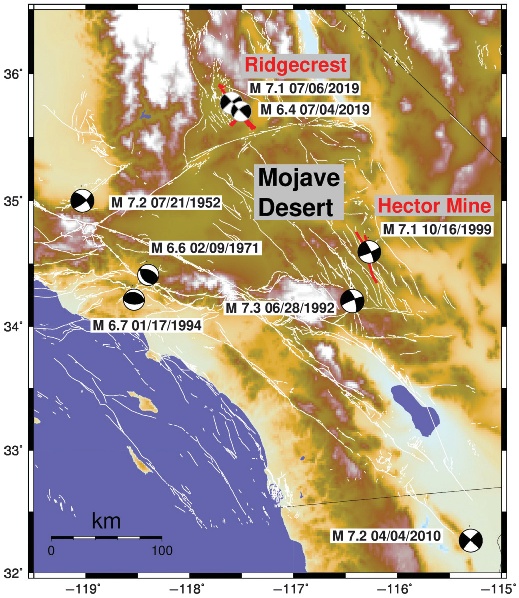
\includegraphics[width=339pt,height=188pt]{Figures/Sample}
				\captionof{figure}{Figure caption goes here. a) Figure caption goes here and provides a brief description of the illustration. Figure caption goes here and explains the main elements shown in the figure. b) Figure caption goes here to indicate how different cases or panels may be interpreted. Figure caption goes here to describe relationships, trends, or schematic features presented. d)  Figure caption goes here.}%
				\label{fig06}%
			\end{minipage}%
		}
	\end{figure}
	
	
	%
	\subsubsection{Sample Third Level Head}
	
	\lipsum[27-29]
	
	%\cite{Abramowitz_1972}
	%\cite{Adiyaman_2001}
	%\cite{Afanasiev_2014}
	%\cite{Afanasiev_2016}
	%\cite{Afanasiev_2019}
	%\cite{Afonso_2013}
	%\cite{AdaSwa97}
	%\cite{Adams_2005}
	%\cite{Agliz_2013}
	
	\begin{itemize}
		\item \verb"\citethisauthor{First, A.,"
			\verb"A. Second, and A. Third}"
		\item \verb"\vol{2}"
		\item \verb"\iss{1}"
		\item \verb"\doi{00.0000/0000000000}"
		\item \verb"\recdate{00 Month 0000}"
	\end{itemize}
	
	\begin{enumerate}
		\item
		List item one goes here to the second row to the second row. List item one goes here to the second row to the second row.
		
		\item
		List item two goes here.
		
		\item
		List item three goes here.
		\begin{itemize}
			\item
			List item one goes here to the second row to the second row. List item one goes here to the second row to the second row.
			
			\item
			List item two goes here.
			
			\item
			List item three goes here.
		\end{itemize}
		\item
		List item one goes here to the second row to the second row. List item one goes here to the second row to the second row.
		
		\item
		List item two goes here.
		
		\item
		List item three goes here.
	\end{enumerate}
	
	
	\section*{STATEMENTS AND DECLARATIONS}
	
	\begin{bmsec}[Supplementary Material]
		All supplementary or supporting information provided by the authors will be published online alongside the main article. When such material is available, it will also be indicated here along with a link to the pdf for downloading.
	\end{bmsec}
	
	\begin{ack}%[CUSTOM ACK HEAD]
		Acknowledge any individuals or organizations that contributed to the research but do not qualify as authors. Include funding sources if not already mentioned.
	\end{ack}
	
	\begin{bmsec}[Author Contributions]
		Provide a detailed account of each author’s contributions to the research and writing of the paper, following the CRediT (Contributor Roles Taxonomy) format (\url{https://credit.niso.org/}). 
		{Author 1}: Conceptualization, Investigation, Methodology, Software, Visualization, Writing - original draft. \textbf{Author 2}: Conceptualization, Investigation, Writing - Review \& Editing, Project administration. \textbf{Author 3}: Conceptualization, Methodology, Writing - Review \& Editing. Author 4: Conceptualization, Investigation. \textbf{Author 5}: Investigation. \textbf{Author 6}: Conceptualization, Writing - Review \& Editing.
	\end{bmsec}
	
	\begin{bmsec}[Conflicts of Interest]
		Disclose any actual or potential conflicts of interest that could influence the research. If there are no conflicts, state this explicitly.\
	\end{bmsec}
	
	\begin{datres}%[CUSTOM HEAD]
		Provide information on the availability of data, code, and protocols. Specify where these materials can be accessed, such as public repositories or upon request. Assigned DOI or other identification numbers, links and any conditions that may be present in order to obtain access should be included. This information should also be included in the references and cited in the text.
		
	\end{datres}
	
	\begin{bmsec}[Funding Received]
		List all sources of funding or financial support received for the research. Include grant numbers and the names of funding organizations.\
	\end{bmsec}
	
	
	\begin{orcaulist}
		\orcaulistitem[0000-0000-0000-0001]{First Author}
		\orcaulistitem[0000-0000-0000-0002]{Second Author}
		\orcaulistitem[0000-0000-0000-0003]{Third Author}
		\orcaulistitem[0000-0000-0000-0004]{Fourth Author}
		\orcaulistitem[0000-0000-0000-0005]{Fifth Author}
		\orcaulistitem[0000-0000-0000-0006]{Sixth Author}
		\orcaulistitem[0000-0000-0000-0007]{Seventh Author}
		\orcaulistitem[0000-0000-0000-0008]{Eighth Author}
	\end{orcaulist}
	
	%%%%%%%%%%%%%%%%%%%%%%%%%%%%%%%%%%%%%%%%%%%%%%%%%%%%%%%%%%%%%%%%%%%%%%%%%
	%%%                      End author content                           %%%
	%%%%%%%%%%%%%%%%%%%%%%%%%%%%%%%%%%%%%%%%%%%%%%%%%%%%%%%%%%%%%%%%%%%%%%%%%
	
	%\bibliographystyle{plainurl}
	%\bibliography{Bibliography}
	
\end{document}
